
%
%  $Description: Author guidelines and sample document in LaTeX 2.09$
%
%  $Author: Gediminas Mazrimas $
%  $Date: 1995/09/15 15:20:59 $
%  $Revision: 1.4 $
%

\documentclass[times, 10pt,twocolumn]{article}
\usepackage{latex8}
\usepackage{times}

% Images includes
\usepackage{graphicx}
\usepackage{float}


%\documentstyle[times,art10,twocolumn,latex8]{article}

%-------------------------------------------------------------------------
% take the % away on next line to produce the final camera-ready version
\pagestyle{empty}

%-------------------------------------------------------------------------
\begin{document}

\title{Animating human model in OpenGL using data from Vicon system}

\author{Algirdas Beinaravicius\\
Aalborg University Copenhagen\\ Computer Vision and Graphics\\algirdux@gmail.com
\and
Gediminas Mazrimas\\
Aalborg University Copenhagen\\ Computer Vision and Graphics\\g.mazrimas@gmail.com
}

\maketitle
\thispagestyle{empty}

\begin{abstract}
   This paper explains how to animate 3D human model in OpenGL,
   using skeleton-driven deformation technique, similar to Linear Blend Skinning
   that computes deformed weighted vertex position, which is calculated using quaternions.
   This helps to avoid some common animation problems, which occur while dealing with
   various human body rigid parts transformations.
   The motion for this animation was captured using motion capture system
   and after processing it and converting to appropriate data format, was ready to use for
   animating 3D human model in lowest programming C++/OpenGL level.

   \textbf{Keywords:} Human animation, Vicon motion capture system, OpenGL, C++, Linear Blend Skinning
\end{abstract}



%-------------------------------------------------------------------------
\Section{Introduction}

Our animation focuses on the most common and partly simple human
body animation technique that uses joint based structure to animate human model. Joint structure,
given their position and orientation, can be thought as human body skeleton.
Animation of the skeleton, when talking about its complexity, is pretty simple,
as it includes only rigid body parts and requires rotations of bones at the joint position.
But when taking in account underlying layer of the skeleton, what we call skin, it becomes more
complicated. This is when linear blend skinning technique comes in use, associating joints to vertices and introducing weights to them. Due to very fast computation speeds, this technique is the most popular
in animation production. On the other hand, while using this simple shape blending technique
to deal with complex transformations various skin deformation problems occur. Typical ones are collapsing elbow, candy-wrapper effect when the arm turns 180 degrees.
Also such a technique doesn't consider many other human body deformations, like stretching or bulging muscles.

%-------------------------------------------------------------------------
\SubSection{Overview}

We present a motion data driven technique of animating a human body model in a program written in C++ programming language and working in an OpenGL environment.
We have two main issues in this work: getting motion data and using it
correctly to animate skeleton and then solving the human model mesh deformation problems.
Using data captured by motion capture system and correctly defined joint structure,
we achieve realistic body movements for our model. Any motion data, which was captured
using same joint structure scheme as ours, can be used for animating that human body model.

After introducing the techniques that we were using in this project (Sections: \emph{\ref{Linear_blend_skinning}} and \emph{\ref{Quaternions}}), explaining about motion data formats and their differences (Section \emph{\ref{Motion_data}}), we give details on how to prepare 3D human body model mesh for our program (Section \emph{\ref{Maya_mesh}}) and how we managed to animate both skeleton and its underlying layer (Section \emph{\ref{Animating_human_body}}).


%-------------------------------------------------------------------------
\SubSection{Previous works}

Linear blend skinning is very widely used technique, but due to its disability to deal with more complex skin deformations, it has many slightly different approaches and modifications for animating human body model. Furthermore, for animating human body model totally different methods are also used, such as anatomy-based ones \cite{ex8}, using different layers to imitate muscle structures, but we won't be going to details of such a technique.

Basic principles of linear blend skinning were described by the game development community \cite{ex13,ex14,ex10} and the artifacts of this technique were discovered very soon \cite{ex15}.
The technique that dealt with some of those issues and set background for linear blend skinning type transformations was introduced in \cite{ex12} and was named as "skeleton subspace deformation". It consider skin deformation as an interpolation problem and radial basis functions are used to interpolate between example skins with different shapes, where a one-to-one vertex correspondence must exist between each pair of examples.

Many other used techniques only extend the previous one. In \cite{ex2} so called "extended linear blend skinning" is introduced. Approaching 180 degrees, the linearly blended matrix becomes degenerate and collapses the skin geometry. This method avoids blending transformations that are so dissimilar by adding extra transformations that properly interpolates
without collapsing. In other paper \cite{ex8} authors introduces non-linear technique to avoid unpleasant defects that are caused by linear shape blending. They achieve that by direct assignment of weights to the
vertices according to its position around the joint. While in \cite{ex10} authors suggest interpolating transformations itself instead of transformed vertex positions. Considering transformations consisting of a translation and rotation, they suggest using a quaternion representation.

To conclude, despite many techniques correcting the problems of linear blend skinning, none of them can fully avoid them. As a result, the traditional linear blend skinning is still widely used in many applications.

%-------------------------------------------------------------------------
\Section{Linear blend skinning}
\label{Linear_blend_skinning}
Linear blend skinning technique is widely used for interactive applications.
It goes by many different names, such as Skeleton Subspace Deformation or SSD or "smooth skinning" in Maya.

The linear blend skinning algorithm works by placing a hierarchical
skeleton inside a static model mesh of a character in
some neutral pose (usually in the da Vinci posture or so called "dress pose").
Then, each vertex is assigned a set of influencing joints and a
blending weight for each influence. Computing the deformation in
some pose involves rigidly transforming each dress pose vertex by
all of its influencing joints. Then the blending weights are used to
combine these rigidly transformed positions.

The deformed vertex position, $ \overline{\textbf{v}} $ is
\begin{center}
$ \overline{\textbf{v}} = \displaystyle\sum_{i=1}^n\emph{w}_{i}M_{i}D_{i}^{-1}\textbf{v}_{d} $
\end{center}
where $w_{i}$ are the influence weights, $v_{d}$ is the dress-pose location of a
particular vertex \textbf{v}, $\emph{M}_{i}$ is the transformation matrix associated with
the $\emph{i}$th influence, and $D_{i}^{-1}$ is the inverse of the dress-pose matrix
associated with the $\emph{i}$th influence. Taken together, $D_{i}^{-1}\textbf{v}_{d}$ represents
the location of \textbf{v$_{d}$} in the local coordinate frame of the $\emph{i}$th influence.

\begin{figure}[H]
  \caption{}
  \centering
  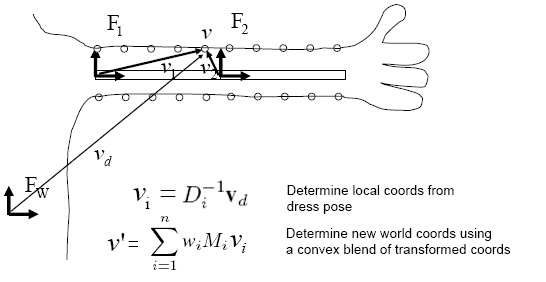
\includegraphics[width=93mm]{images/hand2.jpg}
\end{figure}

Linear blend skinning though has two primary failings.
First, the method is incapable of expressing complex deformations.
Artifacts such as the "candy-wrapper", collapse effect on wrists and
collapsing around bending joints. They
occur because vertices are transformed by linearly interpolated matrices.
If the interpolated matrices are dissimilar as in a rotation of
nearly 180 degrees, the interpolated transformation is degenerate,
so the geometry must collapse.
Second, authoring linear blend skins is difficult and frustrating for users.

Despite its failings, this skinning algorithm is very fast and
widely supported by commercial applications so it remains popular
especially in games and virtual environments.

%-------------------------------------------------------------------------
\Section{Quaternions}
\label{Quaternions}
A quaternion is a mathematical object, consisting of 4 scalars. Quaternions were discovered in 19th century by Irish mathematician Sir William Rowan Hamilton during his search for a way to represent points in space.  Soon after their introduction, quaternions appeared at most of universities as an advanced mathematics subject. Nowadays quaternions find their applications in signal processing, physics, bioinformatics, orbital mechanics as well as computer graphics.
	
In computer graphics Euler angles are known to have the disadvantage of being susceptible to "Gimbal lock" where attempts to rotate an object fail to appear as expected, due to the order in which the rotations are performed. Quaternions are a solution to this problem. Instead of rotating an object through a series of successive rotations, quaternions provide the ability to rotate an object through an arbitrary rotation axis and angle. Though the rotation is still performed by using matrix mathematics, instead of multiplying matrices together, quaternions, representing the axis of rotation, are multiplied together. The final resulting quaternion is then converted to the desired rotation matrix.

As mentioned earlier, a quaternion is four numbers, representing one real dimension and 3 imaginary dimensions. Each of its imaginary dimensions has a unit value of square root of -1 (a complex number). In addition to that, imaginary dimensions are all perpendicular to each other and can be noted as i, j, k. So a quaternion can be represented as follows:
\begin{center}
q = \emph{a} + i$\ast$b + j$\ast$c + k$\ast$d
\end{center}
where \emph{a} is a real dimension representation and b,  c,  d are just scalars.

Since quaternions are mathematical objects, they have a certain algebra with all the addition, subtraction,  multiplication and division operations applied to them. In this section of the report we are going to consider just the quaternion multiplication operation, since this operation is necessary to represent a rotation. All other operations can be found in the references page of the report.

In order to perform a quaternion multiplication, a quaternion's imaginary dimension multiplication has to be described first:

\begin{description}
    \setlength{\itemsep}{0pt}

    \item \emph{i $\ast$ i = j $\ast$ j = k $\ast$ k = -1}
    \item \emph{i $\ast$ j = k}
    \item \emph{j $\ast$ i = -k}
    \item \emph{j $\ast$ k = i}
    \item \emph{k $\ast$ j = -i}
    \item \emph{k $\ast$ i =  j}
    \item \emph{i $\ast$ k = -j}
\end{description}

The multiplication of two quaternions is :

\begin{center}
(a + i$\ast$b + j$\ast$c + k$\ast$d) $\ast$ (e + i$\ast$f + j$\ast$g + k$\ast$h)

$\Updownarrow$

a $\ast$ e + i$\ast$a$\ast$f  + j$\ast$a$\ast$g + k$\ast$a$\ast$h + i$\ast$b$\ast$e - b$\ast$f  + k$\ast$b$\ast$g - j$\ast$ b$\ast$h + j$\ast$e$\ast$c - k$\ast$c$\ast$f - c$\ast$g + i$\ast$c$\ast$h + k$\ast$e$\ast$d + j$\ast$d$\ast$f - i$\ast$d$\ast$g - d$\ast$h

$\Updownarrow$

(a$\ast$e - b$\ast$f - c$\ast$g - d$\ast$h)  + i$\ast$(a$\ast$f + b$\ast$e + c$\ast$h - d$\ast$g) + j$\ast$(a$\ast$g - b$\ast$h + e$\ast$c + d$\ast$f) + k$\ast$(a$\ast$h + b$\ast$g - c$\ast$f + e$\ast$d)
\end{center}

The important thing to notice is that the multiplication of two quaternions is not commutative, so that
\begin{center}
q1 $\ast$ q2 $\neq$ q2 $\ast$ q1
\end{center}

As mentioned above, the multiplication operation,  provides us with the ability to rotate one quaternion by another quaternion. So the rotation of quaternion q1 by quaternion q2 would result in another quaternion q = q2 $\ast$ q1;

Since the representation of a quaternion is quite complex and hard to imagine, it can be interpreted in another way. The x, y, z components of a quaternion can be treated as a representation of rotation axis and a component - as a representation of rotation angle. The relation between actual values and their representations as quaternion's components can be described as:

\begin{itemize}
\item a = $cos(angle / 2)$
\item b =  $axis_x$ $\ast$ $sin(angle / 2)$
\item c = $axis_y$ $\ast$ $sin(angle / 2)$
\item d = $axis_z$ $\ast$ $sin(angle / 2)$
\end{itemize}
where $axis_x$, $axis_y$ and $axis_z$ is a normalized vector, representing the rotation axis.

In order to rotate a 3D point by a quaternion, a rotation matrix $R$ has to be produced:


\[ R = \left( \begin{tiny}\begin{array}{cccc}
a^{2}-b^{2}-c^{2}-d^{2} & 2 \ast b \ast c-2 \ast a \ast d & 2 \ast b \ast d+2 \ast a \ast c & 0 \\
2 \ast b \ast c+2 \ast a \ast d & a^{2}-b^{2}+c^{2}-d^{2} & 2 \ast c \ast d-2 \ast a \ast b & 0 \\
2 \ast b \ast d-2 \ast a \ast c & 2 \ast c \ast d-2 \ast a \ast b & a^{2}-b^{2}c^{2}+d^{2} & 0 \\
0 & 0 & 0 & 1
\end{array}\end{tiny} \right)\]

Instead of calculating the direct rotation matrix, another approach is to calculate back the rotation vector and Eulerian angle from their quaternion representation. The angle can be calculated as:
\begin{description}
	\item angle = arccos(a) $\ast$ 2
\end{description}

The vector can be calculated as:

\begin{description}
    \setlength{\itemsep}{0pt}

    \item sin$_a$ = sqrt(1 - a $\ast$ a);

	\item vector$_x$ = b / sin$_a$
	\item vector$_y$ = c / sin$_a$
	\item vector$_z$ = d / sin$_a$
\end{description}


%-------------------------------------------------------------------------
\Section{Parametric representation of lines in 3D space}
\label{line_in_space_section}

A line is a geometric object, defined by two points A and B. It is infinite in length, passing through the points and extending forever in both directions. A line segment (or just segment) is also defined by two points, its endpoints, but extends only from one endpoint to the other. Although these objects, lines and segments, are very familiar, it is important to describe their parametric representation, as it was one of the solutions, which helped us to implement the linear blend skinning technique.

In order for the linear blend skinning to work, the algorithm, implementing it, has to know exact coordinates of   each vertex, which is going to be affected during the animation of the character. The parametric representation of a line/segment enabled us to find the required vertices, as well as their positions in 3D space.

The parametric representation of a line L can be written as:
\begin{center}
\emph{L(t) = A + b $\ast$ t}
\end{center}
where \emph{b} is a vector: \emph{b = B - A}, \emph{A} is a starting point of a segment and \emph{B} is an ending point of a segment.

This construction gives us a way to name and compute any point along the line \emph{L}. This is done using a parameter \emph{t}, that distinguishes one point on the line from another. As t varies, so does the position of L(t)  along the line.
If \emph{t = 0, L(0)} evaluates to \emph{A}, so at \emph{t = 0} we are at point \emph{A}. At \emph{t = 1} then \emph{L(1) = A + (B - A) = B}. As \emph{t} varies, we add a longer or shorter version of \emph{b} to the point \emph{A}, resulting in a new point along the line. If \emph{t} is larger than 1, this point lies somewhere on the opposite side of \emph{B} from \emph{A}, and when \emph{t} is less than 0, it lies on the opposite side of \emph{A} from \emph{B}. Below is a picture \label{line_in_space} illustrating these facts in a graphical 2D view, although 3D version uses the same ideas.


\begin{figure}[H]
  \caption{Line in space}
  \label{line_in_space}
  \centering
  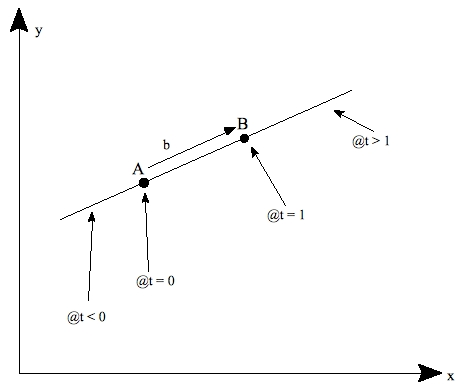
\includegraphics[width=85mm]{images/lines3d.jpg}
\end{figure}

A very useful fact is that \emph{L(t)} lies a fraction \emph{t} of the way between \emph{A} and \emph{B} when \emph{t} lies between 0 and 1. For instance, when t = 0.5 the point L(0.5) is the midpoint between \emph{A} and \emph{B} and when t = 0.3, the point L(0.3) is 30\% of the way from \emph{A} to \emph{B}. This is clear from equation \emph{L(t) = A + b * t} since \emph{$|$ L(t) - A $|$ = $|$ b $|$ * $|$ t $|$} and \emph{$|$ B - A $|$ = $|$ b $|$}, so the value of \emph{$|$ t $|$} is the ratio of the distances \emph{$|$ L(t) - A $|$ to $|$ B - A $|$}.


%-------------------------------------------------------------------------
\Section{Data formats}

%-------------------------------------------------------------------------
\SubSection{Description of Vicon C3D format}

This section is meant to give just a brief introduction to the C3D file format, describing it in an abstract way. A reference to a detailed manual, describing the format, is given in the reference part of this document.

The C3D (Coordinate 3D) file format is a binary data file format originally developed for the AMASS photogrammetry software system, capable of storing 3D data as well as analog data together with all associated parameters for a single measurement trial. Since only the 3D data is of importance, we will not consider analog data in this document. The main advantage of C3D format over other motion capture data formats is that it is able to encapsulate the motion data as well as parameters, describing the  motion data, in a single file. Apart from that, C3D is freely licensed and well documented.

Being a binary file, the C3D file consists of a number of 512-byte blocks. Logically C3D format can be divided into 3 basic sections, each having one or more 512-byte blocks:
\begin{itemize}
\item Header section is the first section of a file. The main purpose of this section is holding a pointer to the start of parameters section. Other parts of this section, is of no particular importance, as usually it consists data, copied from parameters section.

\item The parameters section usually starts at block number 2, although this is not fixed and should not be assumed to be the case for every C3D file. This section contains information about the 3D data stored in the file. The section is extensible, meaning that user can define it's own parameters without  violating the format specification.

\item Data section containing the 3D point coordinates is usually located after the parameters section. This section simply contains sequential frames data. In the case of 3D points (the data is X, Y and Z coordinates).
\end{itemize}

%-------------------------------------------------------------------------
\SubSection{Description of Biovision BVH format}
\label{bvh_description}
The BVH format is an updated version of BioVision�s BVA data format, with the addition of a
hierarchical data structure representing the bones of the skeleton.
The BVH file is an ASCII file and consists of two parts:

\begin{itemize}
\item \emph{Hierarchy} is for storing joint hierarchy and initial pose of the skeleton,
basically joint-to-joint connections and offsets.
\item \emph{Motion} describes the channel motion data for each frame,
that is the movement of individual joints.
\end{itemize}

The \emph{hierarchy} section starts with \emph{root} joint and contains the definition of a joint hierarchy within nested braces like source code written in the C programming language.
Each joint in a \emph{hierarchy} has an \emph{offset} field and a \emph{channels} field.
The \emph{offset} field stores initial \emph{offset} values for each joint with respect to its parent joint.
\emph{Channels} field defines which �channels� of transformation (translation and/or rotation) exist for the joint in
the \emph{motion} data section of the file. The \emph{channels} field also defines the order of transformation. A
\emph{channel} is either x-, y-, or z-translation or local x-, y-, or z-rotation. All the segments are assumed
to be rigid and scaling is not available.
The \emph{end site} field is also available in order to determine body segment end.

In the \emph{motion} section the total number of frames in the animation and the frame
speed in frames-per-second is defined. Every next row then contains data values for all \emph{channels} which were specified in the \emph{hierarchy} section.
The listing order of \emph{motion} values in each row in is assumed to match their listed order from the \emph{hierarchy} section (top down).

There are few drawbacks of the BVH format. One is that it lacks a full definition of the initial pose. Another
drawback is that the format has only translational offsets of children segments from their parents. No
rotational offset can be defined. Moreover, the BVH format is often implemented differently in different
applications, that is, one BVH format that works well in one application may not be interpreted
in another. All the same the format is very flexible and it is relatively easy to edit BVH files.

%-------------------------------------------------------------------------
\SubSection{Description of OBJ format}

OBJ is a geometry definition file format, first developed by Wavefront technologies. The file format is open and has been adopted by most of 3D graphics application vendors. It can be imported/exported from most of 3D modeling tools such as Autodesk's Maya, 3ds Max, Newtek's Lightwave, Blender, etc.  This section of the document provides a  thorough explanation of the most important parts of an object file, with more details provided in the reference page.

An object file can be stored in ASCII (using the ".obj" file extension) or in binary format (using the .MOD extension). The binary format is proprietary and undocumented, so only the ASCII format is described here.

The OBJ file format supports lines, polygons, and free-form curves and surfaces. Lines and polygons are described in terms of their points, while curves and surfaces are defined with control points and other information depending on the type of curve. Since, in our project, lines and polygons were sufficient to represent the model appropriately, only the parameters, concerning, these entities are described below.

The OBJ file is composed of lines of text, each of them starting with a token, which describes the type of the entity being  recorded in that line. Below are listed various tokens, which were of importance in our project:

\begin{itemize}
\item "\#" - a comment line. Lines, starting with "\#" token, are simply skipped by OBJ file readers. For example "\# this is a comment".
\item "g" - a group line. Lines, starting with "g" (group) token, determine the start of a group. "g" token is followed by the group name. For example $"g left_arm"$. In our project each group name corresponded to some body part, described by vertices, textures, normals and polygons.
\item "v" - a vertex line. Lines, starting with "v" (vertex) token, provide the information, concerning vertices. This token is followed by x, y and z coordinates of the vertex. For example "v -0.756447 0.702621 0.047024" is a vertex with coordinates (-0.756447, 0.702621, 0.047024).
\item "vt" - a texture line. Lines, starting with "vt" (vertex texture) token, are recorded with information, concerning textures. "vt" token is followed by x, y and z coordinates of the texture, although only the x and y coordinates are of importance (z coordinate is 0.0). For example "vt 0.487840 0.942165 0.000000".
\item "vn" - a vertex normal line. Lines, starting with "vn" (vertex normal) token, contain information, concerning the normal of a vertex. "vn" token is followed by x, y and z coordinates of the normal. For example "vn 0.149280 -0.186998 -0.240511".
\item "f" - a line, describing face. Lines, starting with "f" (face) token, provide the information, concerning polygons. "f" token is followed by a number of triplets, which is equal to the number of vertices, the polygon has. Each triplet is of a form "int/int/int", where the first "int" is a vertex position in the file, the second "int" is "texture" position in the file and the third "int" is a normal position in the file. For example "f 6/9/6 2/5/2 1/1/1" is a triangle polygon, with vertices 6, 2 and 1, textures 9, 5 and 1 and normals 6, 2 and 1.
\end{itemize}

The above described tokens were of importance in our project, but they are not the only ones that OBJ format allows. The OBJ format specification is much broader and covers such abilities as surface encoding, connectivity between free-form surfaces, rendering attributes. The OBJ specification can be found in the document's reference page.


%-------------------------------------------------------------------------
\Section{Motion capture}

Motion capture (\emph{mocap}) is sampling and recording motion of humans, animals and other various
objects as 3D data. The data can be used to study motion or to animate 3D computer models.
During the motion capture process not only the capturing stage using \emph{mocap} equipment
is very important, as equally important are the preparation and post processing processes.
The whole system must be well calibrated, adjusted and set up, furthermore, after capturing
data needs to be cleaned, edited, and applied to a 3D model.

During this project, for capturing motion data, we used Vicon Motion System,
combined with Vicon IQ 2.5 software running on our systems host pc.
Details about Vicon motion capture system, how we managed to capture and process motion data can be found on the appendix \textbf{\ref{Vicon appendix}}.


%-------------------------------------------------------------------------
\SubSection{Motion data}
\label{Motion_data}

There are various \emph{motion data} storing formats, that mostly depend on what kind of program they
are being used on. Our aim on this project, considering motion data, was to select
the most appropriate data format. After reviewing some examples, the decision was made,
that the best choice for our model animation would be using \emph{BVH} motion data format.
In \emph{BVH} file whole model joint structure is described and motion data is represented as rotations and translations of these joints. This feature allows us to easily animate our skeleton, without any additional calculations.
Only drawback is that our motion capturing is being done using Vicon IQ software,
which is not able to directly export data to BVH file format. At first we need get Vicons' C3D data file
and then convert it to BVH using other 3rd party application.


%-------------------------------------------------------------------------
\Section{Human body mesh model}
\label{Maya_mesh}

Human body mesh model must be selected not only by it's looks and model details,
but also by its position. The model must be in such a position, that in
animating stage you could connect models body parts with your skeleton
and make it move. In this project simple human body mesh was selected with initial T-pose.

%-------------------------------------------------------------------------
\SubSection{Mesh model preparations}

Mesh model is a vital object in animation, looking from the users (viewers) side.
After using all the mathematical theories and different approaches, the final result
highly depends on the mesh being used.
For our project we decided to use whole human body mesh cut in different body parts,
with empty space between these rigid parts, that are later connected to one mesh.
The main issue using this kind of approach, is that you lose details of your body mesh,
so the better solution is using the whole uncut body.

\begin{figure}[H]
  \caption{Mesh model cut in Maya}
  \centering
  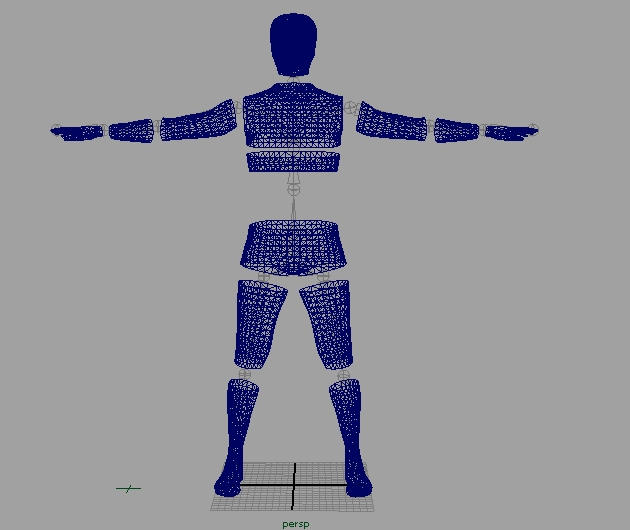
\includegraphics[width=75mm]{images/maya_cut.jpg}
\end{figure}


%-------------------------------------------------------------------------
\Section{Animating human body}
\label{Animating_human_body}

The base of any character animation is its skeleton. A skeleton is a hierarchical structure that let you pose and animate your model. Skeletons are composed of series of joints and bones that form joint hierarchies. Each joint has a number of children joints and one parent. Only the root joint does not have a parent and end-joints don't have children. From a programmers point of view joint hierarchy can be treated as a tree data structure, having a root, nodes and leaves.

\begin{figure}[H]
  \caption{Human body skeleton}
  \centering
  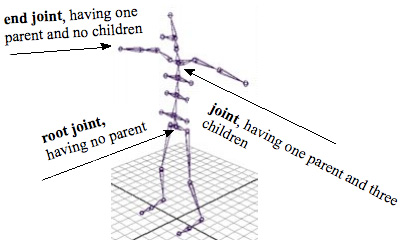
\includegraphics[width=85mm]{images/bodySkeleton.jpg}
\end{figure}

To animate a character, first of all, the animation data has to be applied to characters skeleton (every joint that the skeleton consists of). Generally, the motion of an individual joint consists of translation, rotation and scale components (scaling is usually applied to character's bone). All these components can be merged together to give an overall transform using homogenous coordinates.  If the translation, rotation and scaling is being applied, the overall transformation can be defined as multiplication of corresponding matrices:

\begin{center}
\emph{M = T $\ast$ R $\ast$ S}
\end{center}
where \emph{M} is an overall transformation matrix, \emph{T} is translation matrix, \emph{R} is rotation matrix and \emph{S} is scale matrix.

In our case, only the root joint had translational data, applied to it, whereas all other joints were being applied with rotational data. No scaling data was introduced in our motion capturing data.

For the animation to look correctly, a forward kinematics technique has to be applied. With forward kinematics, you rotate or move individual joints to pose and animate your joint chains. Moving a joint affect's that joint and any joints below it in the hierarchy. For example, if you want a joint chain to reach for a particular location in space, you have to rotate each joint individually so that the joint chain can reach the location. To do this, you rotate and translate the joint chain's parent joint, then the next joint, and so on down the joint chain.

From a more detailed point of view, each joint has a local transformation that describes its orientation within its local coordinate system, which in turn is a subject to its parent's local orientations. To obtain a global matrix transform for a given joint, the local transform needs to be pre-multiplied by it's parents global transform, which itself is  derived by multiplying its local transform with its parent's global transform and so on, until you reach the root joint. For the root joint, the local and the global transforms are the same. The equation below outlines this combination sequence, where \emph{n} is the current joint, whose parent joint is \emph{n - 1}, \emph{n = 0} is the root joint and \emph{M} is the joint's transformation matrix.

\begin{center}
$M^{n}_{global}$ = $\prod^{n}_{i = 0}$ $M^{i}_{local}$
\end{center}

So, for example to get the global transformation of the left ankle joint, the overall transformation sequence might look like this:

\begin{center}
$M_{global\_left\_ankle}$ = $M_{local\_root}$ $\ast$ $M_{local\_left\_hip}$ $\ast$ $M_{local\_left\_knee}$ $\ast$ $M_{local\_left\_ankle}$
\end{center}

%-------------------------------------------------------------------------
\SubSection{Our approach for animating human model}

\SubSection{Preparing the character for animation}
\label{preparing_character}

Our model consists of 18 joints, defined in the BVH data file: Hips (root joint), LeftHip, LeftKnee, LeftAnkle, RightHip, RightKnee, RightAnkle, Chest, Chest2, LeftCollar, LeftShoulder, LeftElbow, LeftWrist, RightCollar, RightShoulder, RightElbow, RightWrist and Neck. All of these joints should be positioned in such a way, that the skeleton is drawn in a T-pose. Below is a picture \ref{our_skeleton} of our skeleton.

\begin{figure}[H]
  \caption{Our skeleton example}
  \label{our_skeleton}
  \centering
  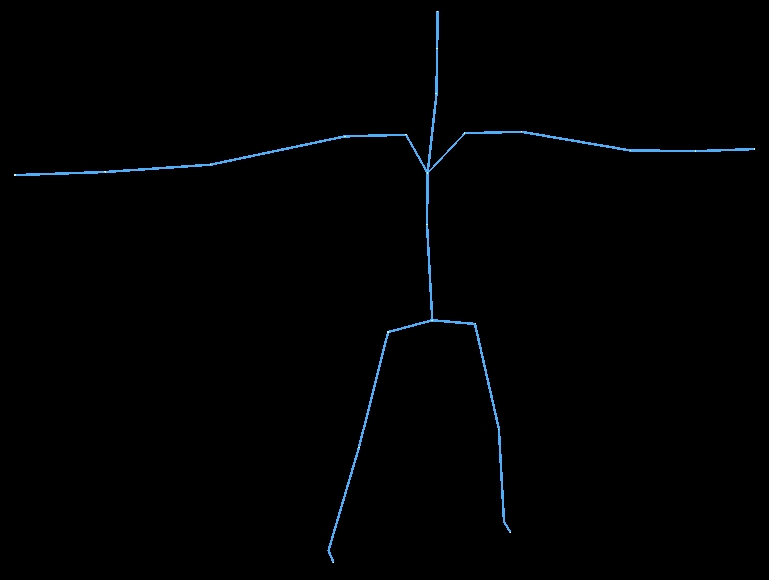
\includegraphics[width=55mm]{images/our_skeleton.jpg}
\end{figure}

The joints, mentioned above, allow our model to be correctly animated in 3D scene, although much detail is not achieved as the movement of fingers and toes is not animated. Each joint has a mesh applied to it, which is not affected by the animation data, except being rotated or translated in the scene. The connection between the meshes is being done automatically during the construction of the character. The algorithm for doing that is:

\begin{enumerate}
\item Find two vertices, belonging to the mesh and its parent mesh, which have the shortest distance of all the vertices.
\item Determine some threshold value, which can be just user defined (for example 5\%). The threshold value determines the longest distance between vertices, belonging to the mesh and its parent.
\item Find all other vertices, which are necessary to connect, by calculating the distance between each of them. If the distance is between the shortest distance and the distance, calculated from the threshold value, then those two vertices have to be connected.
\end{enumerate}

Each connection between the mesh and its parent has subvertices. This is necessary for every joint rotation to look smooth. The more subvertices we have, the smoother the rotation looks. To find positions of subvertices on the connecting line, we apply the parametric representation of a line. To give a better view, of how subvertices are introduced in our model, the image of model's right knee is provided. In the image \ref{our_mesh_connection} you can see two meshes being connected by two connecting lines, each of which has four subvertices. Of course, this picture is provided just for explanatory purposes, the full connection between the meshes should have much more connecting lines.

\begin{figure}[H]
  \caption{Connections between meshes}
  \label{our_mesh_connection}
  \centering
  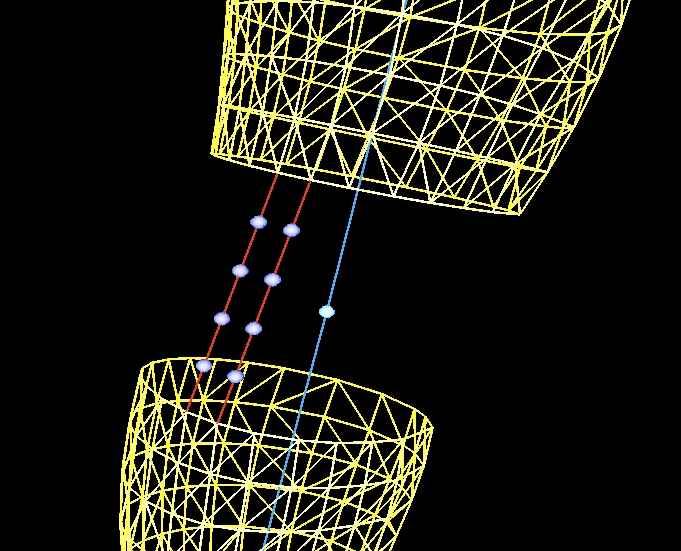
\includegraphics[width=75mm]{images/mesh_connection.jpg}
\end{figure}

Any line function can be written as: \emph{L(t) = A + b*t}, where \emph{A} is the starting point of a line, \emph{b} is a vector, determining the direction of a line and \emph{t} is a parameter value. A more detailed explanation of the parametric representation of the line can be found in documents section \ref{line_in_space_section}.

Since the above mentioned algorithm finds the positions of the first vertex, necessary to connect, (which is letter \emph{A} in the parametric representation of the line) and the second one (let's mark it's position as letter \emph{B}), we can find the direction vector \emph{b = B - A}. Now taking t from 0 to 1 we get the position of the subvertex, which is between \emph{A} and \emph{B}. In fact if we took \emph{t = 0}, from the parametric representation of the line we get the position of vertex \emph{A}, and if we took \emph{t =1}, we get the position of vertex \emph{B}. So to determine the position of the first subvertex on the line, we need to set \emph{t = 1/N}, where \emph{N} is the total number of subvertices. To determine the position of the second subvertex on the line, set \emph{t = 2 * 1/N}. In general, to find the \emph{n}'th subvertex position on the line, we can set

\begin{center}
t = n $\ast$ 1/N
\end{center}

Now to calculate the position of subvertices after rotation, we apply the linear blend skinning technique, which means that each subvertex has some weight (let's mark it as \emph{w}), which influences the angle it has to be rotated. Of course, each subvertex weight could be determined manually (for example, user defined), but we found that it is pretty easy to determine it automatically to get the satisfying overall result.

Let's consider that we have \emph{N} vertices on the connecting line. The joint is being rotated by angle \emph{A}. Each vertex weight \emph{w} is being determined by it's position on the connecting line:

\begin{center}
w = P $\ast$ 1/N
\end{center}
where P is the position on the connecting line.

So the first vertex on the line has the weight \emph{w = 1 $\ast$ 1/N}, while the last vertex on the line has the weight \emph{w =  N $\ast$ 1/N = 1}.

Now, considering the angle each vertex has to be rotated, the first one is rotated by \emph{A $\ast$ 1 $\ast$ 1/N} degrees, while the last one is being rotated by \emph{A $\ast$ N $\ast$  1/N = A} degrees. After rotating all the subvertices, they are being connected to polygons.

\SubSection{Animating the character}
\label{animating_our_character}

Our character is being animated by the data, provided by the Vicon motion capturing system. Motion data is encoded as BVH format file, consisting of  1289 frames (a more detailed explanation about Biovision BVH format is provided in document's section \ref{bvh_description}). Each frame holds rotation values for every joint as well as translation values for root joint in 3D space. Since rotation values are provided as three separate rotations around \emph{X}, \emph{Y} and \emph{Z} axis, quaternions are being used to calculate rotation axis and rotation angle.

For example in the first frame, the root joint is being rotated by -0.66 degrees around \emph{Z} axis, 0.80 degrees around \emph{Y} axis and 171.21 degrees around \emph{X} axis. By applying the mathematics of quaternions, the overall rotation vector is (0.00631242, 0.999959, 0.00653654) and the rotation angle is 171.209 (quaternions are being explained in document's section 3). Since BVH format file provides only local rotations for each joint, to get the global rotation in 3D space, each joint's parent rotation should be taken into account. Considering the previous example, not only the root joint has to be rotated by 171.209 degrees around the rotation axis  (0.00631242, 0.999959, 0.00653654), but all of its children as well.

Since each joint has a mesh applied to it, during the animation, meshes are transformed in 3D scene the same way the joints are translated and rotated. Only the mesh connection has a different approach. In order for the mesh connection to rotate correctly, a linear blend skinning technique is applied, which is explained in more detail in document's section 2.


%-------------------------------------------------------------------------
\Section{Problems}

In this section we give some examples of the problems that occurred during the project.
Some of these problems were solved during the work, while others still need to be seen into.

%-------------------------------------------------------------------------
\SubSection{Initial BVH pose}

During the animation of human skeleton, the initial pose is not important, but when the mesh is considered,
it's all they way around. As our human model was cut into individual parts,
we had to have appropriate initial pose to correctly connect separate meshes. In our case, the appropriate pose was the T-pose. The T-pose was the only pose, which enabled us to find the shortest distance between two meshes and connect them correctly. The detailed way how the meshes are connected is described in section \ref{preparing_character}.

The problem was, that after processing motion data and exporting it to BVH file, the character was not in initial T-pose.
The same problem occurred after trying a number of examples downloaded from the internet. The initial pose was the I-pose instead of the T-pose.
Due to BVH structure, fixing this problem requires the file to be manually edited:

\begin{enumerate}
\item Skeleton structure and joint offsets in BVH file has to be changed to match T pose.
\item All the frame rotations has to be recalculated, as the rotations in BVH file are given from the initial position.
\end{enumerate}

We managed to automate these two steps by using third-party application. After changing the initial pose, the application automatically recalculated frame rotations.

%-------------------------------------------------------------------------
\SubSection{"Exploding knee" problem}

The "exploding knee" problem occurred during the animation, when the overall rotation is being applied as three separate rotations around Z, Y and X axes. This artifact can be seen in figure \ref{knee_explosion}.
During the rotations around Z, Y and X axes in a row, the linear blend skinning algorithm, which we apply to animate connections between meshes, provides faulty results. The solution for this problem was the introduction of quaternions, which enabled us to calculate a unique rotation vector, as well as rotation angle, representing three separate rotations around Z, Y and X axes.

\begin{figure}[H]
  \caption{Knee explosion sequence}
  \label{knee_explosion}
  \centering
  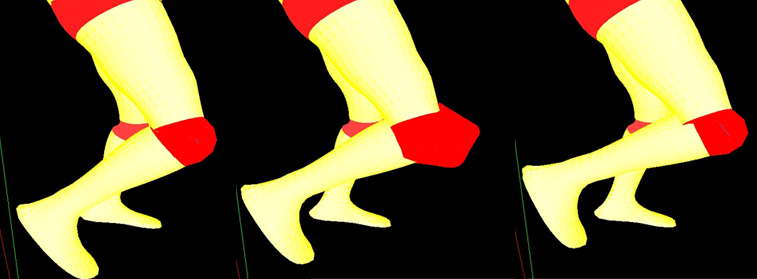
\includegraphics[width=75mm]{images/s_knee_explosion.jpg}
\end{figure}

%-------------------------------------------------------------------------
\SubSection{Mesh connections collapsing on complex deformations}

During the implementation and testing of our linear blend skinning algorithm, only one-axis rotations were considered, which provided really promising results. It can be seen in figure \ref{knee_1axis}.

\begin{figure}[H]
  \caption{Knee rotation by 1 axis}
  \label{knee_1axis}
  \centering
  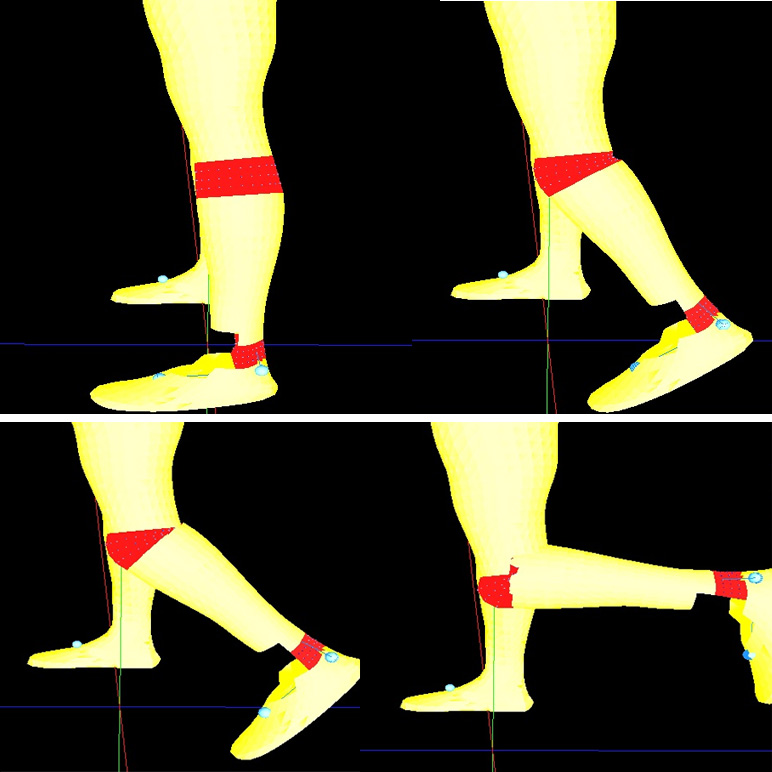
\includegraphics[width=75mm]{images/s_knee_rot1.jpg}
\end{figure}

After introducing a full human body animation and taking data from BVH motion data file, we were provided with rotations around all three axes. Although the application of quaternions enabled us to calculate the rotation vector and angle, representing the transformations around all three axes, the final results were not so smooth as in the testing phase. The results can be seen in figure \ref{knee_3axis}.

\begin{figure}[H]
  \caption{Knee rotation by 3 axis}
  \label{knee_3axis}
  \centering
  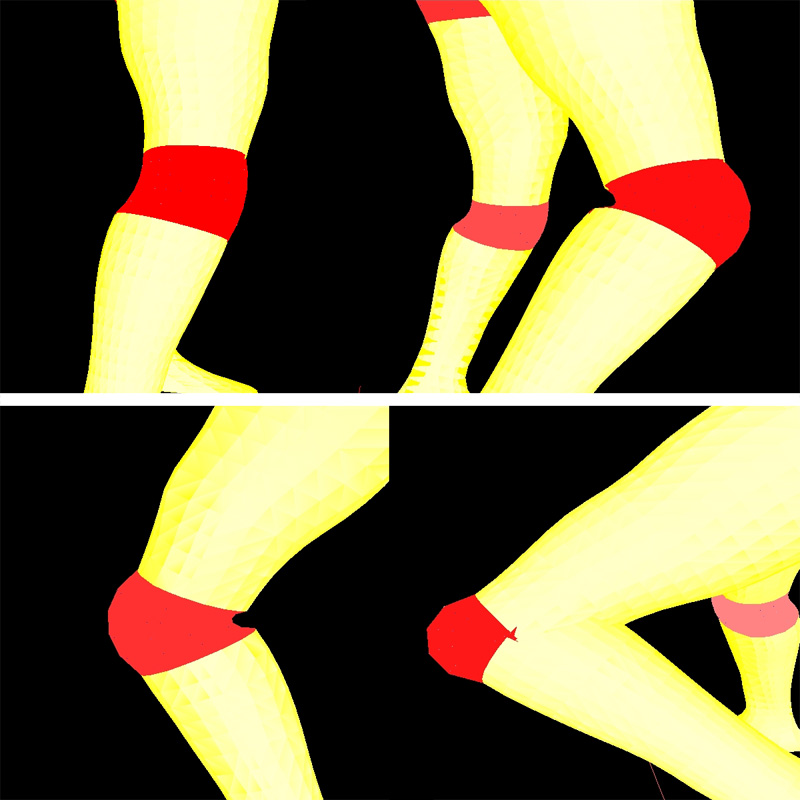
\includegraphics[width=75mm]{images/s_knee.jpg}
\end{figure}

The solution for this problem could be trying different weight distribution for vertices than those we were using.
Other solution, that could give positive results, is cutting out smaller bits of the model.

%-------------------------------------------------------------------------
\Section{Conclusion}

 The aim of this project was to animate human model using data from the Vicon motion capturing system. For the animation to look smooth, the linear blend skinning technique was chosen. To realize the linear blend skinning algorithm correctly, merits of quaternions were applied as well. Although linear blend skinning is very popular among game developers and other 3D graphics communities, the technique is not perfect. The linear blend skinning implementation in our project showed up with many problems. Usually most of them are solved by manually assigning different weights for each vertex, but this way requires user interruption, whereas our idea was to automatically determine the correct weights.
 
 All in all, our project succeeded in animating the human model in 3D scene. The main goals were reached, though improvements are necessary at some areas.

%-------------------------------------------------------------------------
\SubSection{Future work}
Possible further improvements:
\begin{enumerate}
    \item More detailed animation (moving fingers sand toes);
    \item Detailed facial animation;
    \item Improved animation around joint areas. Reconsidering the implementation of linear blend skinning technique;
    \item Live streaming to our animating program (straight from motion capture system to animation in OpenGL);
    \item Other skin deformations (stretching/bulging muscles).
\end{enumerate}

%-------------------------------------------------------------------------
\clearpage
\newpage

\appendix

\section{Details of using Vicon motion system}
\label{Vicon appendix}
\input vicon_appendix.tex

\clearpage
\newpage

%-------------------------------------------------------------------------
\nocite{ex1,ex2,ex3,ex4,ex5,ex6,ex7,ex8,ex9,ex10,ex11,ex12,ex13,ex14,ex15}
\bibliographystyle{latex8}
\bibliography{latex8}

\end{document}


